\documentclass[journal=jacsat,manuscript=article]{achemso}

% Image-related packages
\usepackage{graphicx}
\usepackage{subcaption}
\usepackage[export]{adjustbox}
\usepackage{wrapfig}
\usepackage{hyperref}  % Add the hyperref package

\newcommand*\mycommand[1]{\texttt{\emph{#1}}}

\author{Nayanika Das}
\affiliation[UVicUCC]{Computational Biochemistry and Biophysics Lab, Research Group on Bioinformatics and Bioimaging (BI$^2$), Department of Biosciences, Universitat de Vic - Universitat Central de Catalunya, 08500 Vic, Spain}
\author{Gunjan Paul}
\affiliation
\author{Vijay Baladhye}
\affiliation[SPPU]{Savitribai Phule Pune University, Pune, India}
\author{Jordi Villà-Freixa}
\email{jordi.villa@uvic.cat}
\affiliation[UVicUCC]{Computational Biochemistry and Biophysics Lab, Research Group on Bioinformatics and Bioimaging (BI$^2$), Department of Biosciences, Universitat de Vic - Universitat Central de Catalunya, 08500 Vic, Spain}
\alsoaffiliation{IRIS-CC}

\title[Computational analysis of GPX6 activation free energy]
  {Computational analysis of the evolution of glutathione peroxidase 6 (GPX6) activation free energy}

\abbreviations{IR,NMR,UV}
\keywords{Ancestral enzyme reconstruction, enzyme design, empirical valence bond, free energy calculations}

\begin{document}

\begin{abstract}
Outstanding success in computational protein design has been achieved in recent years by combining machine learning approaches with physicochemical properties analysis of the explored variants. Despite these efforts, however, less success has been obtained in designing good computational protocols for optimization of enzyme activity. Here we propose the use of the Empirical Valence Bond method to evaluate free energies of activation of enzyme variants to obtain reasonable mutational pathways leading to a functionally optimized protein. In particular, we propose a method that explores a lower free energy difference pathway for the directed evolution of enzymes based on EVB activation free energies. To test the idea, we study the hypothetical connectivity of the selenocysteine-containing human glutathione peroxidase 6 protein (GPX6) into its ortholog cysteine-containing mouse GPX6. We show how it is possible to find a mutational pathway connecting the two protein sequences and structures that provide the empirical barriers for the first step of the GPX6-catalyzed reaction. Moreover, this protocol offers the potential for addressing complex issues such as epistasis in enzyme engineering, further enhancing its utility in enzyme optimization.
\end{abstract}

\section{Introduction} \label{sec:intro}  % Label the Introduction section for linking
Selenium (Se), in the form of selenocysteine (Sec, U—the 21st amino acid) occurs in 25 proteins in the human proteome. Insertion of Sec into a protein is much more complicated than the other 20 amino acids because a UGA stop codon must be recoded as a sense codon for Sec \cite{hondal_differing_2011}. The complexity of this process signifies that Sec must fulfill a chemical function that exerts biological pressure on the genome to maintain the Sec-insertion machinery \cite{hondal_differing_2011,cardey_selenocysteine_2007}. The view of Sec as a sophisticated innovation implies that for each occurrence of Sec in an enzyme there is a unique and specific reason for the use of Se to enhance the enzymatic reaction relative to that of S\cite{hondal_differing_2011}. The view of Sec as a sophisticated innovation implies that for each occurrence of Sec in an enzyme there is a unique and specific reason for the use of Se to enhance the enzymatic reaction relative to that of S \cite{hondal_differing_2011}. This view also implies that since Se “speeds reactions” Sec should have widely substituted for Cys in enzymes, which clearly has not occurred. Specific reasons for the usage of Sec might include the enhanced nucleophilic character of Se relative to S, or another might be the much lower pKa of a selenol relative to that of a thiol \cite{hondal_differing_2011}.

Selenium (Se), in the form of selenocysteine (Sec, U—the 21st amino acid) occurs in 25 proteins in the human proteome. Under physiological conditions, inorganic or organic Se is mostly metabolized into selenocysteine (Sec), an amino acid that is then inserted into the primary structure of peptide chains to form selenoproteins \cite{}. Insertion of Sec into a protein is much more complicated than the other 20 amino acids because a UGA stop codon must be recoded as a sense codon for Sec \cite{hondal_differing_2011}. The micronutrient Se is either metabolized through the trans-selenation pathway or via reduction by thioredoxin reductases (TXNRDs) in the presence of glutathione (GSH), depending on the dietary chemical form ingested\cite{}.  The complexity of this process signifies that Sec must fulfill a chemical function that exerts biological pressure on the genome to maintain the Sec-insertion machinery \cite{hondal_differing_2011,cardey_selenocysteine_2007}. The view of Sec as a sophisticated innovation implies that for each occurrence of Sec in an enzyme there is a unique and specific reason for the use of Se to enhance the enzymatic reaction relative to that of S \cite{hondal_differing_2011}. Specific reasons for the usage of Sec might include the enhanced nucleophilic character of Se relative to S, or another might be the much lower pKa of a selenol relative to that of a thiol\cite{hondal_differing_2011}. Besides the fundamental role organoselenides have in organic catalysis, particularly in oxidations of substrates by $H_{2} O_{2}$, selenium-mediated redox reactions are key steps in biological processes related to oxidative stress control and cell signaling \cite{14}. Glutathione peroxidase from class 1 (GPX1, EC 1.11.1.9) is a selenoprotein which protects cells from oxidative damage by catalyzing the reduction of $H_{2} O_{2}$.

Although the catalytic triad of glutathione peroxidase (GPX) has been well recognized, there has been little evidence for the relevance of the interactions among the triad amino acid, i.e. selenocysteine (U), glutamine (Q), and tryptophan (W). Hence, the mechanism of has been studied in various aspects. A catalytic mechanism proposed for GPX3 by Prabhakar et al. based on DFT calculations has the resting state of Sec as selenol, In the first part of this reaction, hydrogen peroxide coordinates to the active site of the enzyme and the proton tranfer is happening to the oxygen atom of Gln residue \cite{prabhakar_elucidation_2005,prabhakar_is_2006}. While another study demonstrated that the ionized selenolate state of Sec in GPX1 is the favorable form for the reduction of hydroperoxide substrates where they modeled the first reaction step of the redox cycle of based on the proposed GPX1-\({\ Sec^-}\)- Arg177 mechanism [8]. Flohe et al. [6]\cite{orian_selenocysteine_2015} explored the mechanism in two different ways wherein the selenocysteine proton moves via water to the indol nitrogen of the Trp residue and then the hydrogen peroxide and with the result of formation of  the products are instantly, without any measurable activation energy. And on the other hand they also explored another path where the hydrogen peroxide was added in the first step of the redox step of the conversion of SeH (selenol) to selenolate ion \({\ Sec^-}\)\cite{flohe_glutathione_2022,orian_selenocysteine_2015}. The most feasible mechanism that we followed here is the SeH-Gln83 by using the implementation of the DFT calculated and experimental values from the reference reaction \cite{prabhakar_is_2006}. 

\begin{figure}
  \caption{Proposed mechanism for GPX6 (ND, what is the source? Did you create this figure? Is it obtained directly from another article? Can you reference it appropriately?) If yours, leave it here but generate an appropriate figure and not a screenshot. If the figure is from others, we may still adapt it from the original and leave it in the introduction.}
   \label{fgr:example}
   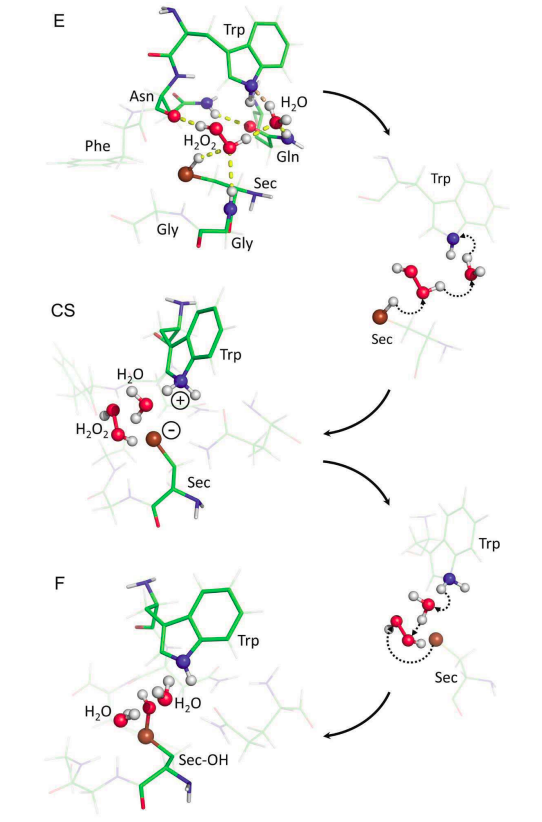
\includegraphics[width=\linewidth]{figures/mechanism.png} 
 \label{fig:mechanism}
 \end{figure}

 \begin{figure}
  \caption{Gibbs free energies of the intermediates and transition states in gas phase and in condensed phase (ND: Are these Gibbs free energy profiles? Or energy values?; can you properly add the citation of the article this was taken from?). If these are your results, leave them here. If they come from another paper, specify it elsewhere, and not in the results or at least compare them with your calculations here. Finally, generate a table with the data once you know what you want to show, and not a screenshot.}
   \label{fgr:etable}
   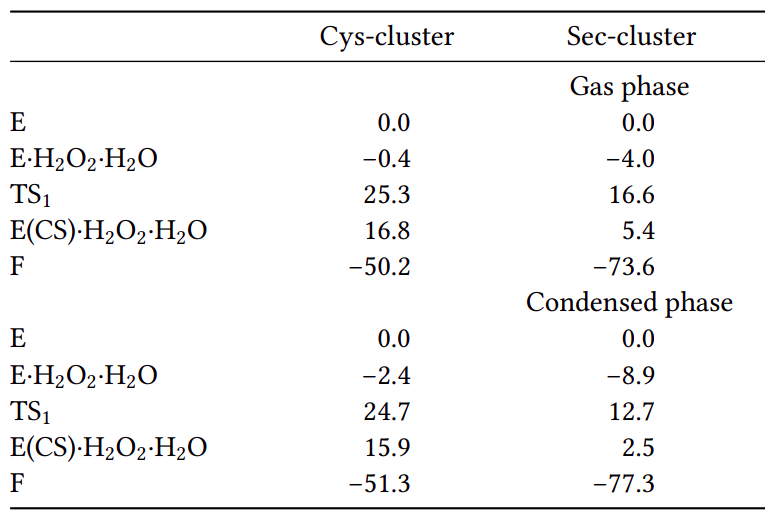
\includegraphics[width=\linewidth]{figures/Etable.png} 
 \label{fig:etable}
 \end{figure}

 \begin{figure}
  \caption{Eprofile (ND same questions as in the previous table? What are these? Are they the same numbers from the previous table? Can you add the citation?) }
   \label{fgr:eprofile}
   \includegraphics[width=\linewidth]{figures/Eprofile.png} 
 \label{fig:eprofile}
 \end{figure}

Catalytic residues are largely conserved in enzymes as they lower the activation energy of reactions and thereby can increase enzymatic turnover \cite{rees_ancient_2024}. Mutations in these active sites typically reduce catalytic activity. In this study we focus on selenoprotein Glutathione Peroxidase 6 (GPX6), while exploring the replacement in several mammalian lineages of the rare amino acid selenocysteine (Sec) for Cysteine (Cys). GPXSec activity classically reduces hydroperoxides, particularly hydrogen and lipid peroxides, with glutathione (GSH) as a cofactor. GPXCys containing proteins act on alternative substrates for peroxidation and may have additional functions, including signalling and oxidative protein folding. Thus, all GPX proteins may protect cells from oxidative stress. The goal of this article was to calculate the activation free energy barrier for the Glutathione Peroxidase 6 active site cysteine-containing mouse and selenocysteine-containing human enzyme using Empirical Valence Bond simulation, in order to determine the significant barrier difference with the change in the active site residue from Cys/Sec and the variants obtained from the previous phylogenetic study \cite{rees_ancient_2024}. Moreover, showing analysis on the effect of the catalytic activity of both due to variants imposing environmental changes inside the protein.  

You can link to the Introduction section by adding this line anywhere in the document (e.g., in your Table of Contents or a citation list):

```latex
\hyperref[sec:intro]{Introduction}
